\chapter{Background estimation}
\label{chap:backgrounds}

%\chapterquote{}{}

\section{Introduction}

The processes used to extract the \PZ invisible width are \IZvv and \IZll. The \IZll process is selected by the \dimuplusjets and \dieleplusjets regions and receives small contributions from background processes, predominantly diboson, as a result of the signal enhancement from the invariant mass selection. Therefore, these backgrounds are estimated from MC after the corrections discussed in Chap.~\ref{chap:simulation-corrections} are applied. Furthermore, the distinction between the \IDYll and \IZll processes requires an estimate of the contribution of the \Pgstar background as well as the interference between \PZ and \Pgstar. With the invariant mass selection, the \Pgstar and interference contributions are percent-level and hence estimated directly from MC simulations where the \PZ and \Pgstar contributions are subsequently turned off in the event generation. Meanwhile, the \IZvv process is collected in the \metplusjets region which is contaminated by the \IWlv decay where the lepton is out of acceptance or a misidentified \Ptauh.  This \IWlv background is estimated by a data-driven control region method. The remaining backgrounds are significantly smaller and estimated from MC, apart from the QCD multijet background which, although small, is estimated with a data-driven method because of large uncertainties associated with the QCD multijet prediction in MC. All these estimation methods are discussed in this chapter.

The estimation methods are performed in orthogonal control regions to the \metplusjets and \diellplusjets signal regions. However, decisions on further categorisation within the regions is closely aligned to the signal regions.  Although the determination of the \PZ invisible width requires the overall event yield for the \IZvv and \IZll processes, the \recoil is divided into bins to exploit the background and systematic uncertainty dependence on this parameter. The chosen bin widths are approximately equivalent to the resolution of the \recoil with an open-ended final bin, as detailed in Tab.~\ref{tab:met-bins}.

\begin{table}[htb]
    \centering
    \begin{tabular}{ccccccc}
        $200$--$220$ & $220$--$250$ & $250$--$280$ & $280$--$310$ & $310$--$340$ & $340$--$370$ & $370$--$400$ \\
        $400$--$430$ & $430$--$470$ & $470$--$510$ & $510$--$550$ & $550$--$590$ & $590$--$640$ & $640$--$690$ \\
        $690$--$740$ & $740$--$790$ & $790$--$840$ & $840$--$900$ & $900$--$960$ & $960$--$1020$ & $1020$--$1090$ \\
        $1090$--$1160$ & $1160$--$1250$ & $1250$--$1400$ & $1400$--$\inf$
    \end{tabular}
    \caption[Recoil bins.]{
        Division of the recoil, in GeV, into 25 bins for the background estimation and \PZ invisible width extraction. Exploiting the shape of the recoil distribution exposes regions with larger signal to background ratios and various systematic uncertainty contributions.
    }
    \label{tab:met-bins}
\end{table}

\section{\IWlv prediction}\label{sec:wjets-prediction}

The \IWlv process contribution in the \metplusjets region is estimated from an orthogonal control region defined by the reconstruction and selection of a single lepton, rather than vetoing all leptons. Two control regions are defined: the \muplusjets and \eleplusjets, both are used in this estimation method as a source of well-reconstructed leptons and complement each other.  These regions are linked to the \metplusjets region through the transfer factor method, discussed in the following section. In addition to the two control regions, the \tauplusjets is defined as a validation region to test the use of muon and electron final states to primarily predict the $\tau$-lepton decay of the \IWlv process.


\subsection{\muplusjets control region}

The \muplusjets control region provides the primary measurement for the data-driven estimate of \IWlv in the \metplusjets region. It differs from this region by requiring a single well-reconstructed muon in the final state along with a transverse invariant mass between the muon and the \ptmiss between $30$ and $\SI{125}{GeV}$. The kinematic distributions for this region are shown in Fig.~\ref{fig:muplusjets}.
%
\begin{figure}[htb]
    \centering
    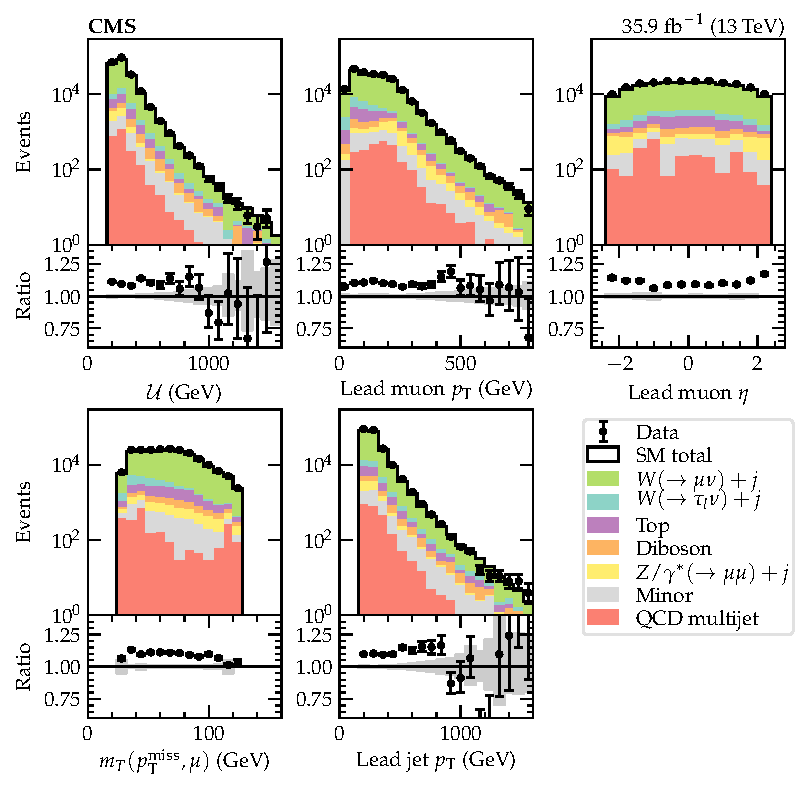
\includegraphics{chapters/042_backgrounds/images/singlemuon_dists.pdf}
    \caption[Single muon final state kinematics.]{
        Distributions of kinematic variables within the \muplusjets region. The ratio of data to MC is shown in the lower sub-panels along with the statistical uncertainty associated with the MC prediction, without any systematic uncertainties. Processes with the largest cross sections are labelled with a grouping of the smallest contributions into the `minor' background.
    }
    \label{fig:muplusjets}
\end{figure}
%
The most prominent processes include the signal of interest, \IWmvj ($82.1\%$), along with backgrounds from: \IWlv with a $\tau$-lepton decaying into a muon ($5.4\%$); $t$-quark production ($5.3\%$) and subsequent decay into a muon, jets and neutrinos; diboson production ($2.0\%$); Drell-Yan production of dimuons ($2.0\%$) with one muon out of acceptance or misreconstructed; QCD multijet ($1.3\%$) and other processes ($1.9\%$). The shape of the data and MC distributions are in agreement. Dependence, for instance, with the lead muon $\eta$ is covered by systematic uncertainties which are larger in the endcaps where the particle flux is greater and the magnetic field is more complex. However, there is a significant discrepancy of $10\%$ between the data and MC normalisation, currently attributed to a normalisation issue with the \IWj production\footnote{This issue has been identified as a problematic cross section deviating from the true theory prediction by about $10\%$ across the full boson \pt range for the \IWj process.}. The analysis is designed to be robust against incorrect normalisations with the \IVj process through data-driven measurements. This is investigated further by inspecting the \eleplusjets control region.


\subsection{\eleplusjets control region}

The selection for the \eleplusjets control region is closely aligned to the \muplusjets to provide a complementary measurement of the \IWlvj process. However, the additional selection ${\ptmiss>\SI{100}{GeV}}$ reduces QCD multijet contamination within this region and the statistical power to measure the \IWlvj process. The kinematic distributions of this region are shown in Fig.~\ref{fig:eleplusjets} where the same $10\%$ discrepancy between the normalisation in data and MC is observed, although the shapes of the distributions are in good agreement.
%
\begin{figure}[htb]
    \centering
    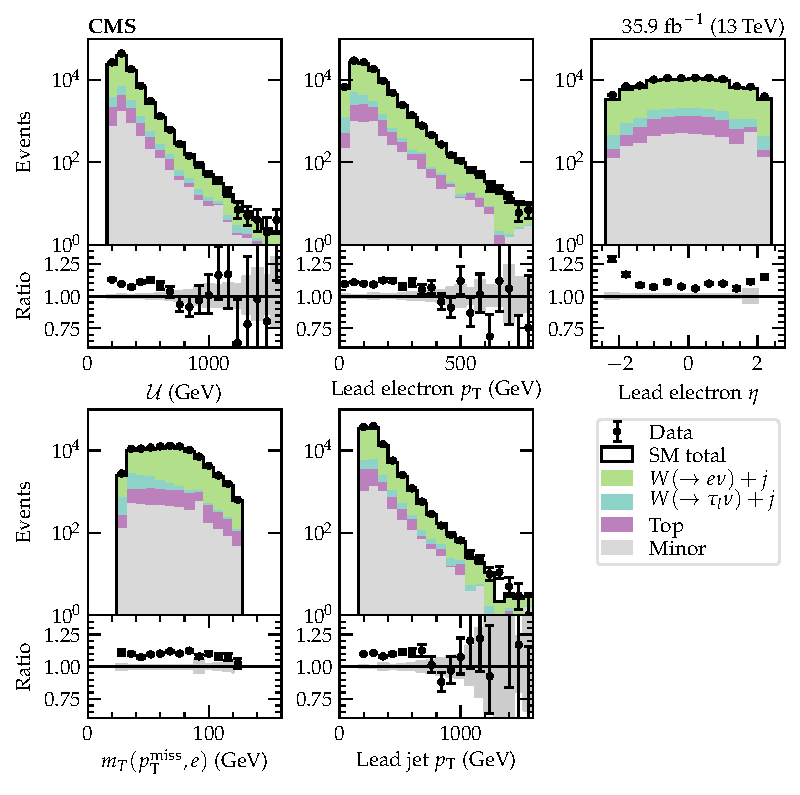
\includegraphics{chapters/042_backgrounds/images/singleele_dists.pdf}
    \caption[Single electron final state kinematics.]{
        Kinematic variable distributions of the \eleplusjets control region. The ratio of data to MC gives an indication of their agreement within statistical uncertainties on both the data and MC. However, no systematic uncertainties are included. The most prominent processes are the electron ($81.1\%$) and $\tau$-lepton ($7.4\%$) decays of the \PW boson, with subsequently smaller contributions from $t$-quark production ($6.6\%$) and other `minor' backgrounds which include diboson, \IDYee and QCD multijet processes.
    }
    \label{fig:eleplusjets}
\end{figure}
%
Therefore, the normalisation is not attributed to the muon or electron reconstruction and identification or the trigger since they differ for the \muplusjets and \eleplusjets regions. This supports the original hypothesis of a normalisation issue with the \IWj process. Under this hypothesis the normalisation is expected to persist into the \metplusjets region, scaled down by the relative contribution of the \IWj process. Therefore, the data-driven estimate of this process is vital for an accurate background prediction. The \tauplusjets region is explored to further support or refute this hypothesis. The different background composition compared to Fig.~\ref{fig:muplusjets} is driven by the additional \ptmiss selection in the \eleplusjets region.


\subsection{\tauplusjets validation region}

The \tauplusjets validation region is more aligned with the \metplusjets region than the \muplusjets or \eleplusjets control regions since no well-reconstructed lepton exists in the final state, instead a hadronic cluster is tagged as the decay product of a $\tau$-lepton. However, as shown in Fig.~\ref{fig:tauplusjets}, this region receives a substantial contribution from other hadronic final states with jets mistagged as a \Ptauh and a lower sample size due to the \Ptauh-tagging efficiency with a large associated uncertainty.
%
\begin{figure}[htb]
    \centering
    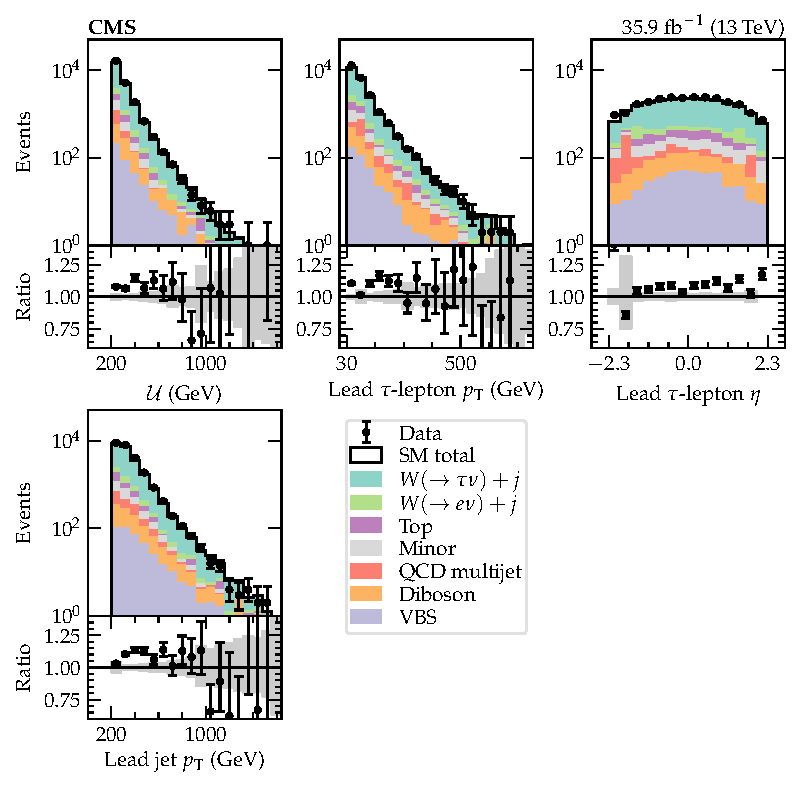
\includegraphics{chapters/042_backgrounds/images/singletau_dists.pdf}
    \caption[Single hadronic $\tau$-lepton final state kinematics.]{
        Kinematic distributions for the \tauplusjets validation region. The \IWj process is dominant with the $\tau$-lepton ($73.4\%$) and electron ($6.9\%$) decays, with subsequently smaller backgrounds from $t$-quark production ($5.7\%$); QCD multijet ($3.6\%$); diboson production ($3.2\%$); vector boson scattering, VBS ($1.8\%$); and other contributions grouped into the `minor' background.
    }
    \label{fig:tauplusjets}
\end{figure}
%
Therefore, for the purpose of measuring the \IWj process, the \tauplusjets region does not provide a similar precision to the \muplusjets and \eleplusjets regions. However, as a validation region it supports the normalisation offset associated with the \IWj process at $8\%$, with the shapes of the kinematic distribution in good agreement, within uncertainties, between data and MC.


\subsection{Systematic uncertainties}

The \IWj background estimation is based on a data-driven estimate to improve the MC prediction. The systematic uncertainties associated with the MC predictions, most notably from limited knowledge of selection efficiencies, impact this estimation. The full set of systematic uncertainties affecting the background estimation is as follows.

\begin{itemize}
    \item All \textbf{theory uncertainties} discussed in Sec.~\ref{sec:theory-corrections}.
    \item \textbf{Veto efficiencies} associated to uncertain corrections in vetoing $b$-jets, photons and \Ptauh-leptons. The photons have two associated uncertainties: identification and pixel seed veto efficiencies.
    \item \textbf{Proton beam uncertainties} such as the luminosity measurement ($\SI{2.5}{\%}$) and the pileup profile.
    \item \textbf{Detector-based uncertainties} due to online issues whilst recording data. The most significant uncertainty is due to the ECAL timing issue.
    \item \textbf{Trigger efficiencies} as described in Sec.~\ref{sec:met-trigger-efficiency} and \ref{sec:electron-trigger-efficiency}. The \ptmiss trigger efficiency uncertainty is split into three sources: reference trigger, muon multiplicity and independent region. The reference trigger uncertainty is correlated between all regions whereas the muon multiplicity is split into the $0\ \mu$, $1\ \mu$ and $2\ \mu$ regions and the independent region systematic is uncorrelated between all regions.
    \item \textbf{Muon efficiency uncertainties} associated to veto and selection muon identification and isolation with an uncorrelated statistical and systematic component.
    \item \textbf{Electron efficiency uncertainties} associated to veto and selection electron identification and reconstruction.
    \item \textbf{Jet energy correction uncertainties} determined by varying the scale (JES) and resolution (JER) of jet energies.
    \item \textbf{Unclustered energy uncertainty} encoding the impact of energy deposits, below the clustering threshold, on \ptmiss.
\end{itemize}


\subsection{Transfer factor method}

The transfer factor method is based on applying correction factors, determined from control regions, to improve background predictions in a signal region whilst reducing the systematic uncertainties associated with this estimation.  The \IWj prediction in the \metplusjets region, $N_{\mathrm{pred}}^{\metplusjets}(\IWj)$, is determined from the \ellplusjets regions as
%
\begin{equation}
    N_{\mathrm{pred}}^{\metplusjets}(\IWj) = \frac{N_{\mathrm{MC}}^{\metplusjets}(\IWj)}{N_{\mathrm{MC}}^{\ellplusjets}(\IWj)} \left(N_{\mathrm{obs}}^{\ellplusjets} - N_{\mathrm{MC}}^{\ellplusjets}(\mathrm{bkgs.})\right)\ ,
\end{equation}
%
where $N_{\mathrm{MC}}^{\metplusjets}(\IWj)$ and $N_{\mathrm{MC}}^{\ellplusjets}(\IWj)$ are the MC predictions for the \IWj process in the \metplusjets and \ellplusjets regions, respectively; $N_{obs}^{\ellplusjets}$ is the observed number of events in data for the \ellplusjets regions, and $N_{\mathrm{MC}}^{\ellplusjets}(\mathrm{bkgs.})$ is the MC prediction for the backgrounds (processes other than \IWj) in the \ellplusjets region. The transfer factor is given by the ratio
%
\begin{equation}
    t_{\ellplusjets}^{\metplusjets}(\IWj) = \frac{N_{\mathrm{MC}}^{\metplusjets}(\IWj)}{N_{\mathrm{MC}}^{\ellplusjets}(\IWj)}\ .
\end{equation}
%
Systematic uncertainties common in both the numerator and denominator typically cancel, reducing the systematic uncertainty associated with the transfer factor, with respect to the individual MC predictions. In practice, the transfer factor method is implemented within the likelihood formalism (App.~\ref{app:likelihood}) by scaling the \IWj process in the signal and control regions by a common unconstrained parameter $r_{\PW}$ determined from a simultaneous fit to the data in the \metplusjets and \ellplusjets region. Here, the likelihood is given by the product over all \recoil bins with two poisson terms for the \metplusjets and \ellplusjets region with the expectation values
%
\begin{equation}
    r_{\PZ}s_{\IZvv}^{\metplusjets}(\bm{\theta},\phi^{\metplusjets})%
    + r_{\PW}s_{\IWlv}^{\metplusjets}(\bm{\theta},\phi^{\muplusjets})%
    + b^{\metplusjets}(\bm{\theta},\phi^{\metplusjets})
\end{equation}
%
and
%
\begin{equation}\label{eq:ellplusjets-expectation}
    r_{\PW}s_{\IWlv}^{\ellplusjets}(\bm{\theta},\phi^{\ellplusjets})%
    + b^{\ellplusjets}(\bm{\theta},\phi^{\ellplusjets})\ ,
\end{equation}
%
respectively. The \IZvv contribution in the \metplusjets region, $s_{\IZvv}$, is scaled by the parameter of interest $r_{\PZ}$; and similarly by $r_{\PW}$ for the \IWlv process $s_{\IWlv}$. The remaining backgrounds, $b$, and all other processes depend on the gaussian constrained, $\bm{\theta}$, and poisson constrained MC statistical, $\phi$, nuisance parameters. Superscripts denote the parameter's associated region. The scaling parameters $r_\PZ$ and $r_\PW$ are correlated across all \recoil bins, and estimated from a fit to the data. Prior to the fit the MC predictions and the transfer factors are inspected, as shown in Fig.~\ref{fig:tfs_emu_sr}.

\begin{figure}[htb]
    \centering
    \begin{subfigure}[b]{\textwidth}
        \centering
        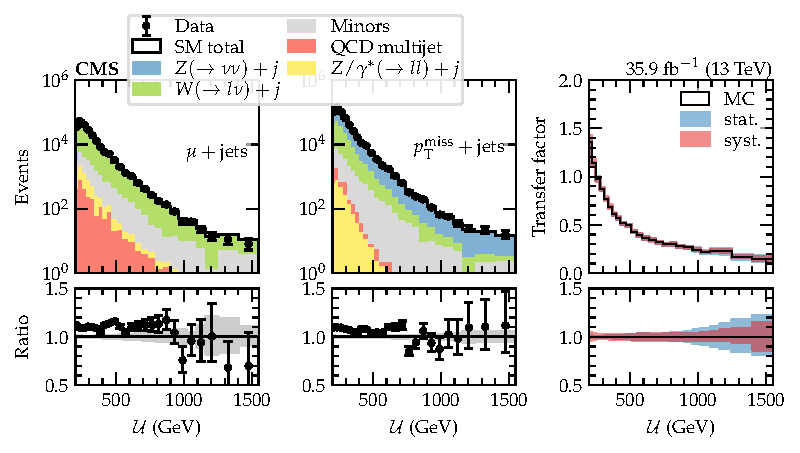
\includegraphics{chapters/042_backgrounds/images/tf_mu_sr.pdf}
        \caption{Transfer factor for \IWj from the \muplusjets to \metplusjets region.}
        \label{subfiga:tfs_emu_sr}
    \end{subfigure}
    \\
    \begin{subfigure}[b]{\textwidth}
        \centering
        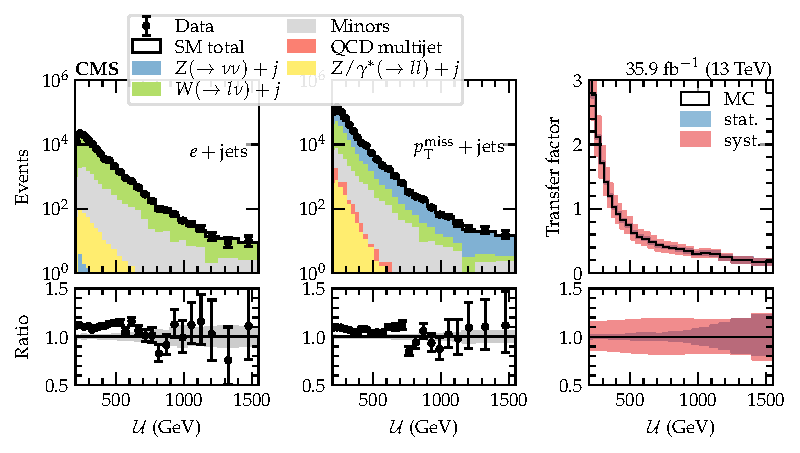
\includegraphics{chapters/042_backgrounds/images/tf_e_sr.pdf}
        \caption{Transfer factor for \IWj from the \eleplusjets to \metplusjets region.}
        \label{subfigb:tfs_emu_sr}
    \end{subfigure}
    \caption[Muon and electron transfer factors into the signal region]{
        Distributions of the \recoil variable in the \muplusjets, \eleplusjets and \metplusjets with the transfer factor determined from the \IWj MC estimates. The transfer factor includes the uncertainties associated with the limited number of generated MC events and systematic uncertainties from all sources whereas the kinematic distributions only include the statistical uncertainties. The distributions also include the analysis relevant processes.
    }
    \label{fig:tfs_emu_sr}
\end{figure}

The transfer factor is a steeply falling distribution where leptons from \PW decays are more likely to be below the \pt acceptance, misreconstructed or misidentified with a lower recoil. However, the \pt of the lepton increases with the recoil and is significantly harder to miss, resulting in the transfer factor tending to zero. Furthermore, the transfer factor is larger for the \eleplusjets predictor rather than \muplusjets because of the tighter selection and lower reconstruction efficiency associated with the electrons.

The systematic uncertainties associated with the \muplusjets and \eleplusjets transfer factor are split into the theoretical and experimental uncertainties. The relative systematic uncertainties associated with the transfer factor $t_{\muplusjets}^{\metplusjets}(\IWj)$ and $t_{\eleplusjets}^{\metplusjets}(\IWj)$ are shown in Figs.~\ref{fig:tf-systs-muplusjets-1}--\ref{fig:tf-systs-eleplusjets-2}.
%
\begin{figure}
    \centering
    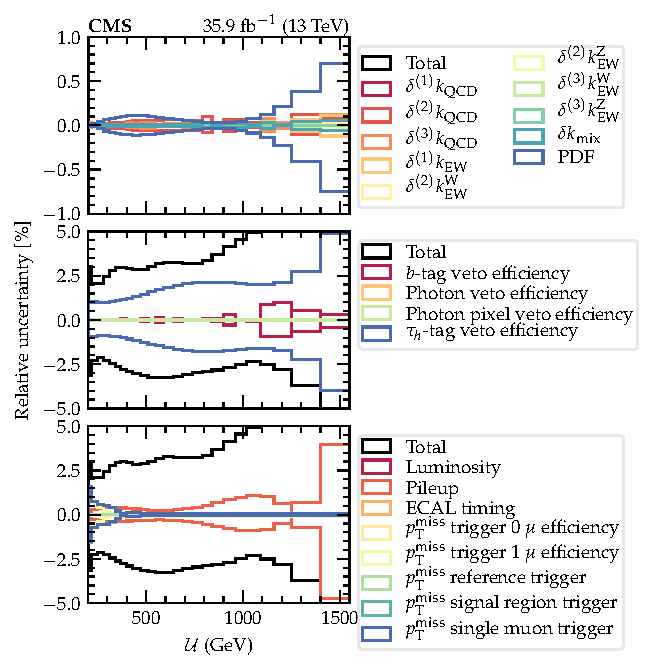
\includegraphics{chapters/042_backgrounds/images/tf_wj_mu_met_systs1.pdf}
    \caption[Theoretical uncertainty on the transfer factors]{
        Relative systematic uncertainties (\%) on the \IWj transfer factor for the \metplusjets region predicted by the \muplusjets control region. The uppermost panel includes all the theoretical uncertainties, while the others include experimental uncertainties. The total depicted in all represents all uncertainties summed in quadrature.
    }
    \label{fig:tf-systs-muplusjets-1}
\end{figure}
%
\begin{figure}
    \centering
    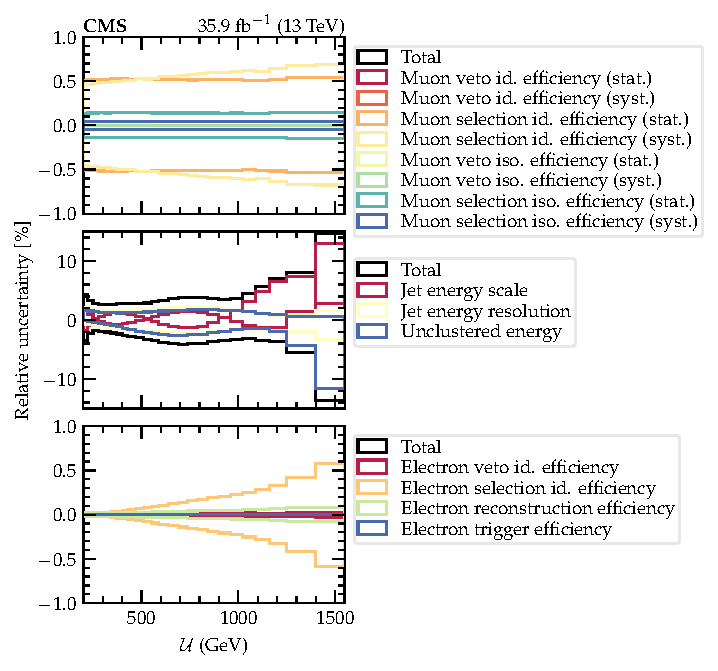
\includegraphics{chapters/042_backgrounds/images/tf_wj_mu_met_systs2.pdf}
    \caption[Object-based uncertainties on the transfer factors]{
        Additional object-based systematic uncertainties to Fig.~\ref{fig:tf-systs-muplusjets-1}.
    }
    \label{fig:tf-systs-muplusjets-2}
\end{figure}
%
\begin{figure}
    \centering
    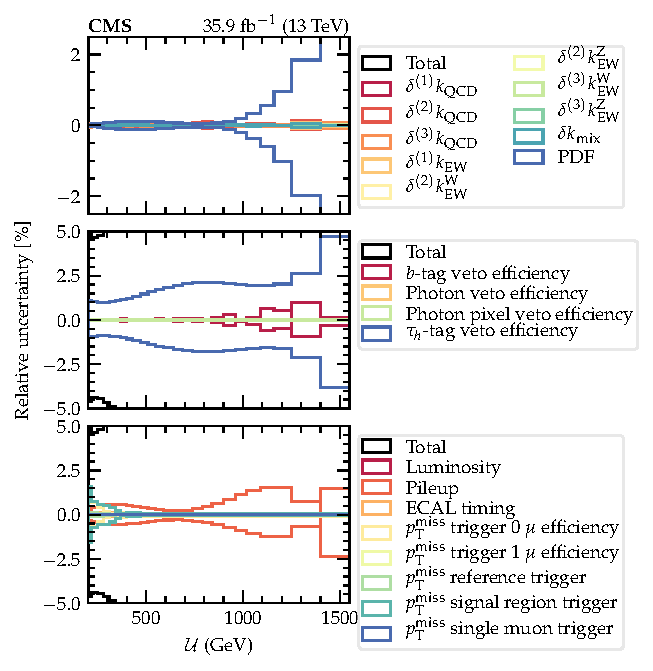
\includegraphics{chapters/042_backgrounds/images/tf_wj_ele_met_systs1.pdf}
    \caption[Theoretical uncertainty on the transfer factors]{
        Relative systematic uncertainties (\%) on the \IWj transfer factor for the \metplusjets region predicted by the \muplusjets control region. The uppermost panel includes all the theoretical uncertainties, while the others include experimental uncertainties. The total depicted in all represents all uncertainties summed in quadrature.
    }
    \label{fig:tf-systs-eleplusjets-1}
\end{figure}
%
\begin{figure}
    \centering
    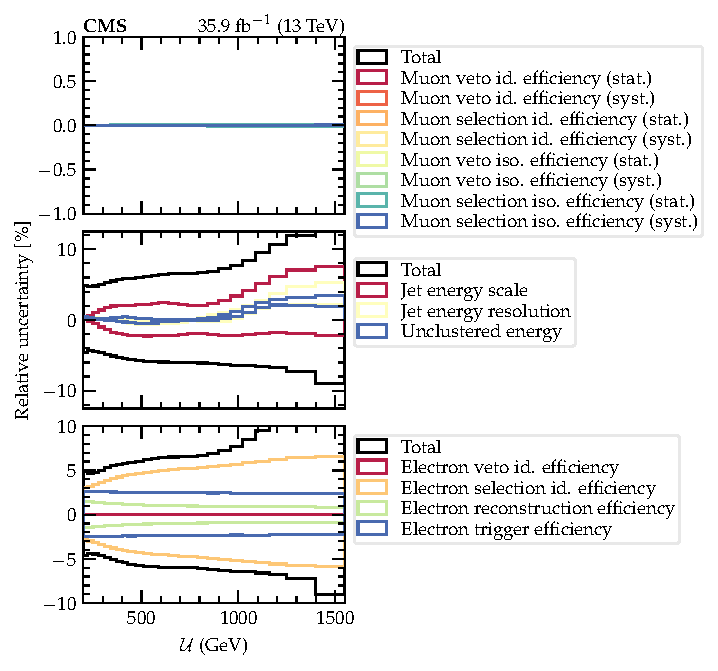
\includegraphics{chapters/042_backgrounds/images/tf_wj_ele_met_systs2.pdf}
    \caption[Object-based uncertainties on the transfer factors]{
        Additional object-based systematic uncertainties to Fig.~\ref{fig:tf-systs-eleplusjets-1}.
    }
    \label{fig:tf-systs-eleplusjets-2}
\end{figure}
%
The theoretical uncertainties primarily cancel as they affect the \IWj process equally in the \metplusjets and \muplusjets regions. However, the parton distribution function (PDF) uncertainty does not completely cancel as different partons initiate the interaction as a result of kinematic sculpting by requirements on muon \pt and $\eta$ which are not applied in the \metplusjets region. Nevertheless these contributions are small in comparison to the experimental uncertainties. The dominant systematic uncertainties include the jet energy scale and resolution, unclustered energy uncertainty, $\Ptauh$-tag veto efficiency and pileup reweighting uncertainty with large contributions from the \ptmiss trigger efficiency for ${\recoil<\SI{250}{GeV}}$. The jet energy uncertainties have a complex contribution to the \recoil variable, depending on alignment and jets below thresholds, resulting in the asymmetric relative uncertainty on the transfer factor. Furthermore, the alternative templates representing the $\pm 1\sigma$ variations in the jet energy correction uncertainties are statistically limited in their precision, whereas they are assumed to be precise within the likelihood fit. Therefore, a smoothing technique is used to remove statistical fluctuations (App.~\ref{app:likelihood}).

A set of validation studies are performed to test the transfer factor and the extrapolation involved in predicting the \IWj process in the \metplusjets regions from the \IWj process in the \ellplusjets region.


\subsection{Validation}

Several aspects of the transfer factor approach are tested to determine if additional systematic uncertainties are required to cover mismodelling, undercoverage or bias in the MC prediction. The major background in the \metplusjets region consists of the \IWj process ($34.7\%$), split by decay mode: electron ($6.3\%$), leptonic decay of the $\tau$-lepton ($6.9\%$), muon ($9.2\%$) and \Ptauh-lepton ($12.3\%$). The data-driven estimate of these processes is performed from the \muplusjets and \eleplusjets control regions.  The leptonic decay of the $\tau$-lepton is similar to the electron and muon decay modes, with a typically broader \recoil distribution. However, the \Ptauh-lepton decay mode differs by being a fully hadronic final state.  Therefore, the validation tests are as follows: test the grouping of the muon and electron decay modes, test the extrapolation of the muon and electron decay modes to predict the \Ptauh-lepton decay mode, and a test of the effects of \PW polarisation.

The first test verifies the consistency of the \muplusjets and \eleplusjets region to validate their combination in measuring the \IWj process. A simultaneous likelihood fit is performed between both regions with expected values given by Eq.~\ref{eq:ellplusjets-expectation}. Two additional unconstrained parameters are applied to the \IWj prediction in the \eleplusjets region to extract the normalisation, $r_e$, and shape, $\beta_e$, difference between both regions. Therefore, the expectation for the \IWj process in the \eleplusjets region is modified to
%
\begin{equation}
    r_{\PW}s_{\IWlv}^{\eleplusjets}\mapsto \left(r_e + \beta_{e}(\recoil/\langle\recoil\rangle-1)\right)r_{\PW}s_{\IWlv}^{\eleplusjets}\ ,
\end{equation}
%
where $\langle \mathcal{U} \rangle$ is the weighted average of the \recoil distribution to scale $\beta_e$ to a dimensionless parameter, $\beta_e$ varies the shape of the \IWj process in the \eleplusjets region linearly with respect to the \muplusjets region. Perfect consistency between both regions corresponds to $r_e=1$ and $\beta_e=0$. The postfit\footnote{Postfit refers to the set of best fit values, or parameters determined at these values, estimated from a fit to the data. Conversely, prefit refers to the set of initial values, prior to a fit to the data. The values are typically chosen such that the prefit distributions correspond to the MC predictions.} values for the parameters of interest are
%
\begin{align}
    r_e & = 0.95^{+0.05}_{-0.05}\qquad \mathrm{and}\nonumber\\
    \beta_e & = -0.020^{+0.024}_{-0.023}\ .
\end{align}
%
Both are in agreement with a consistent muon and electron channel. The quality of the fit is inspected through the postfit results for the nuisance parameters along with their impact on the parameter of interest $r_e$, shown in Fig.~\ref{fig:fit_tf_mu_e_wj_impacts}.
%
\begin{figure}[htb]
    \centering
    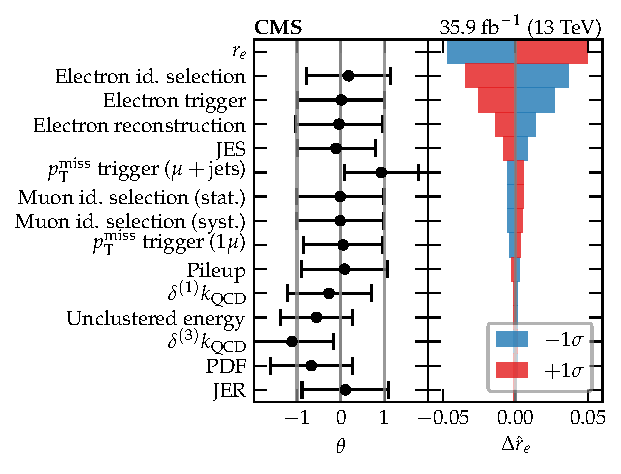
\includegraphics{chapters/042_backgrounds/images/impacts_tfmu2ewj.pdf}
    \caption[Nuisance parameters from a simultaneous fit to the muon and electron control regions]{
        Result of a simultaneous fit between the \muplusjets and \eleplusjets region to extract the scale and shape difference between the muon and electron decay modes. The postfit values for the nuisance parameters and their uncertainties are shown as $\theta$ as well as the impact of fixing the nuisance parameters at the $+1\sigma$ and $-1\sigma$ values to determine the effect on the parameter of interest, $\Delta \hat{r}_e$. The set of parameters is restricted to the top $15$, in order of impact on the parameter of interest. The $\theta$ value for $r_e$ is omitted since it is not a nuisance parameter, instead it is included as a reference for its uncertainty shown in $\Delta \hat{r}_e$.
    }
    \label{fig:fit_tf_mu_e_wj_impacts}
\end{figure}
%
The postfit nuisance parameters are within a satisfactory limit without significant deviations from the $|\theta|<1$ region. Therefore, discrepancies between the data and prediction are covered by the unconstrained parameters, with a slight deviation in the low recoil \muplusjets region covered by the \ptmiss trigger efficiency systematic. The systematic uncertainties with the largest impact on the scale $r_e$ are the electron identification, trigger and reconstruction efficiency uncertainties. The postfit distributions, Fig.~\ref{fig:fit_tf_mu_e_wj_postfit}, show the consistency between the postfit prediction and the data.
%
\begin{figure}[htb]
    \centering
    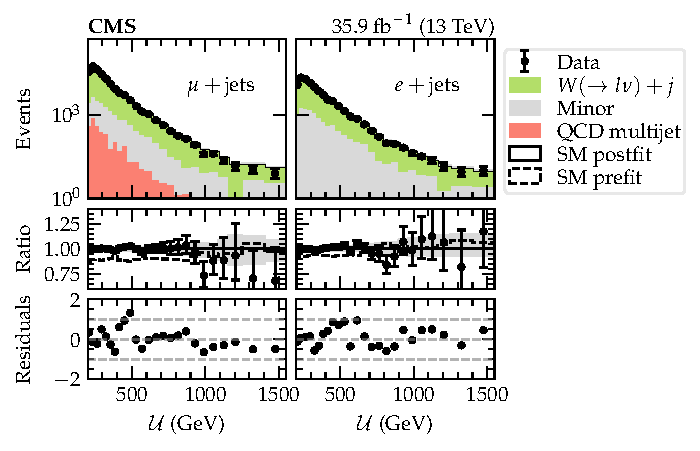
\includegraphics{chapters/042_backgrounds/images/postfit_tfmu2ewj.pdf}
    \caption[Recoil distributions in the muon and electron control regions after applying the transfer factors]{
        Distributions of the \recoil in the \muplusjets and \eleplusjets with the prefit inputs as well as the postfit results along with its uncertainty. The upper panel shows the results in terms of the event counts with the postfit background composition, while the middle panel shows the ratio to the postfit value and the residuals are defined by the difference between the data and postfit result, normalised by the statistical and systematic uncertainties summed in quadrature.
    }
    \label{fig:fit_tf_mu_e_wj_postfit}
\end{figure}
%
A good agreement between the data and postfit values supports the results of the fit and the consistency of the \muplusjets and \eleplusjets. Therefore, the current \IWj prediction formed from a mixture of muon and electron decay modes is kept without the need for additional systematic uncertainties to cover further mismodelling, even though the selections and background compositions differ.

The next validation is a test of the consistency between the \muplusjets and \eleplusjets with the \tauplusjets region. This probes the extrapolation performed by the transfer factor method, using the \muplusjets and \eleplusjets region to predict the \IWj process in the \metplusjets region which mostly consists of \Ptauh decays of the \PW boson. This test is performed in a similar way to the previous test, however, the \IWj process in the \muplusjets and \eleplusjets regions are scaled by a single unconstrained parameter $r_W$, whereas the equivalent process in the \tauplusjets region is scaled by
%
\begin{equation}
    \left(r_\tau + \beta_\tau (\mathcal{U}/\langle \mathcal{U} \rangle - 1)\right) r_\PW s_{\IWlv}^{\tauplusjets}\ .
\end{equation}
%
The postfit values of these parameters are
%
\begin{align}
    r_\tau & = 1.04^{+0.07}_{-0.06}\qquad\mathrm{and} \nonumber\\
    \beta_\tau & = -0.008^{+0.046}_{-0.047}\ .
\end{align}
%
Again, these values show a consistency in the shape and normalisation of the \ellplusjets and \tauplusjets channels. The nuisance parameters and their impacts on the parameter of interest $r_\tau$ is shown in Fig.~\ref{fig:fit_tf_mue_t_wj_impacts}.
%
\begin{figure}[htb]
    \centering
    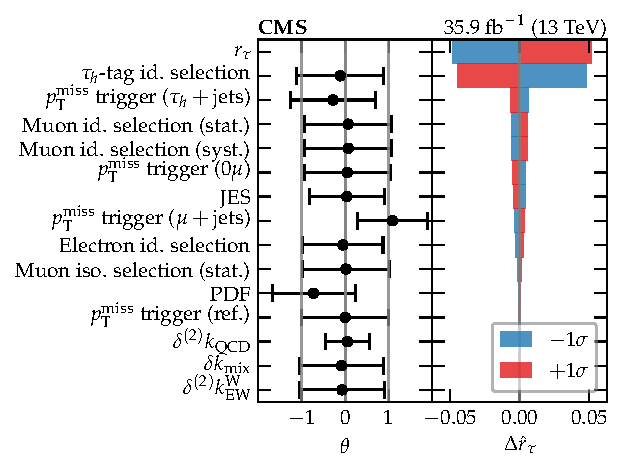
\includegraphics{chapters/042_backgrounds/images/impacts_tfmue2twj.pdf}
    \caption[Nuisance parameters from a fit with the transfer factor method from the muon and electron control regions to the $\tau$-lepton validation region.]{
        Postfit nuisance parameters and impact on $r_\tau$ from a simultaneous fit between the \muplusjets, \eleplusjets and \tauplusjets region. The format is aligned with Fig.~\ref{fig:fit_tf_mu_e_wj_impacts}.
    }
    \label{fig:fit_tf_mue_t_wj_impacts}
\end{figure}
%
Although the \tauplusjets suffers from a smaller sample size compared to the \muplusjets and \eleplusjets regions, the most dominant source of uncertainty comes from the \Ptauh-tag identification uncertainty, albeit unsurprisingly.  The pull\footnote{A pull on a postfit nuisance parameter refers to the deviation of the postfit value from its prefit.} on the \ptmiss trigger efficiency is consistent with the first test since the same region is used, with an enhanced pull on the PDF uncertainties, although within the satisfactory region. The associated \recoil distributions from this fit are shown in Fig.~\ref{fig:fit_tf_mue_t_wj_postfit}.
%
\begin{figure}[htb]
    \centering
    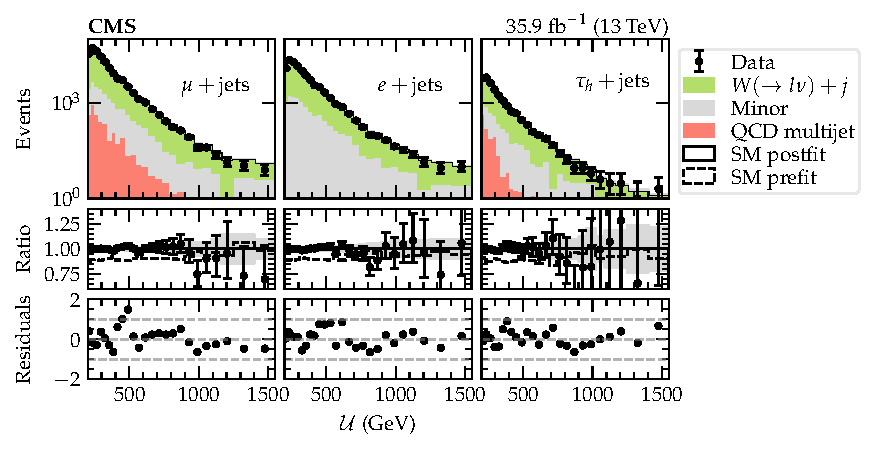
\includegraphics{chapters/042_backgrounds/images/postfit_tfmue2twj.pdf}
    \caption[Recoil distributions corrected by the transfer factor from the muon and electron control regions to the $\tau$-lepton validation region.]{
        Recoil distributions for the \muplusjets, \eleplusjets and \tauplusjets region from a fit to the data to test the extrapolation of a well-reconstructed muon or electron to predict the rate of \Ptauh decays from the \IWj process. The axis definitions are aligned with Fig.~\ref{fig:fit_tf_mu_e_wj_postfit}.
    }
    \label{fig:fit_tf_mue_t_wj_postfit}
\end{figure}
%
The \muplusjets and \eleplusjets regions are similar to those shown in Fig.~\ref{fig:fit_tf_mu_e_wj_postfit} because the \tauplusjets region does not provide any additional information. Furthermore, the data and postfit result in the \tauplusjets region are in excellent agreement. This is partially by design from the unconstrained parameters $r_\tau$ and $\beta_\tau$ used to extract the consistency between the various channels.

The final validation tests the extrapolation performed from the different admixture of $\PW^{\pm}$ polarisation states between the \ellplusjets and \metplusjets regions. The different admixture is a result of the typically softer $\ell^+$ \pt compared to $\ell^-$ \pt to maintain the left-handed chiral state of the associated neutrino (and right-handed anti-neutrino) \cite{Bern:2011ie}. This validation is performed with a similar method, however, the \muplusjets is split into two regions: $\mu^- +\mathrm{jets}$ is used to predict the \IWj process in the $\mu^+ + \mathrm{jets}$, hence testing this extrapolation. Since the admixture difference is significantly smaller than the difference between these two regions, any result discrepancies will have a reduced impact on the \IWj prediction. In this fit, both regions are scaled by the unconstrained parameter $r_\PW$, with two additional normalisation and shape parameters applied to the $\mu^+ +\mathrm{jets}$ region as
%
\begin{equation}
    \left(r_{\mu^+} + \beta_{\mu^+}(\mathcal{U}/\langle\mathcal{U}\rangle-1)\right)r_\PW s_{\IWlv}^{\mu^++\mathrm{jets}}\ .
\end{equation}
%
The postfit values for the parameters from a fit to the data are
%
\begin{align}
    r_{\mu^+} & = 0.976^{+0.013}_{-0.013}\qquad\mathrm{and}\nonumber\\
    \beta_{\mu^+} & = 0.007^{+0.025}_{-0.024}\ .
\end{align}
%
The uncertainty on the normalisation parameter is noticeably smaller than previous validation tests as a result of the closer alignment between both regions leading to further cancellations with the transfer factor method. The null hypothesis of consistent shape and normalisation between the \mupplusjets and \munplusjets is within the $95\%$ confidence level\footnote{A null hypothesis is typically excluded if it falls outside of the $95\%$ confidence interval.} with an excellent shape agreement and a normalisation near the boundary, although within the consistent limits. The postfit nuisance parameters and their impacts on the unconstrained parameter $r_{\mu^+}$ are shown in Fig.~\ref{fig:fit_tf_mup_mun_wj_impacts}.
%
\begin{figure}[htb]
    \centering
    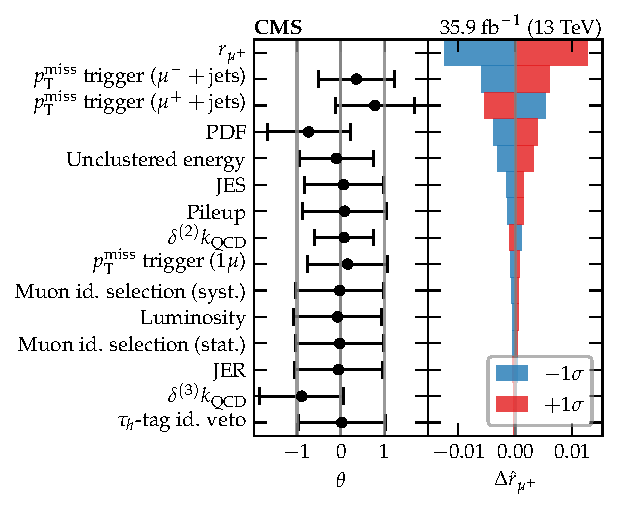
\includegraphics{chapters/042_backgrounds/images/impacts_tfmup2munwj.pdf}
    \caption[Nuisance parameters from a fit to the positive and negative muon control regions.]{
        Postfit nuisance parameters from a simultaneous fit to the \mupplusjets and \munplusjets regions to extract the shape and normalisation difference. The impacts on the $r_{\mu^+}$ parameter are shown. The format is aligned with Fig.~\ref{fig:fit_tf_mu_e_wj_impacts}. The enhanced postfit uncertainty on the jet energy resolution is a result of its asymmetric uncertainties evident from its $\Delta \hat{r}_{\mu^+}$ impact.
    }
    \label{fig:fit_tf_mup_mun_wj_impacts}
\end{figure}
%
The pulls are consistent with previous results including the \muplusjets region, without any significant deviations from the prefit values. No significant constraints are estimated for the nuisance parameters, other than a slight constraint on the $\delta^{(2)}k_{\mathrm{QCD}}$, also seen in Fig.~\ref{fig:fit_tf_mu_e_wj_impacts}. This nuisance parameter is associated to the higher-order QCD corrections discussed in Sec.~\ref{sec:theory-corrections}. In particular, this systematic uncertainty is included to account for unknown shape dependencies from the choice of the factorisation and renormalisation scale. However, this introduces a partial double-counting of the uncertainty on $\delta^{(1)}k_{\mathrm{QCD}}$, the normalisation effect of the choice of factorisation and renormalisation scales \cite{Lindert:2017olm}. Moreover, the postfit results are in excellent agreement with the data, as shown in Fig.~\ref{fig:fit_tf_mup_mun_wj_postfit}.
%
\begin{figure}[htb]
    \centering
    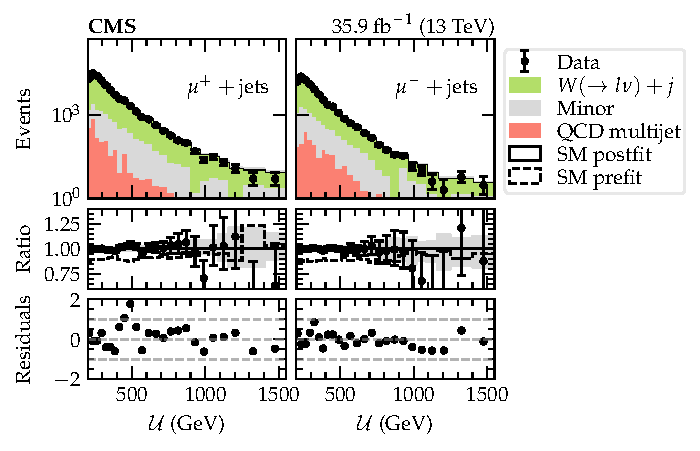
\includegraphics{chapters/042_backgrounds/images/postfit_tfmup2munwj.pdf}
    \caption[Recoil distributions after a fit to the positive and negative muon control regions]{
        Postfit \recoil distributions in the simultaneous fit between the \mupplusjets and \munplusjets regions. The axis definitions are aligned with Fig.~\ref{fig:fit_tf_mu_e_wj_postfit}.
    }
    \label{fig:fit_tf_mup_mun_wj_postfit}
\end{figure}

The validation tests show a consistency between the three lepton-based regions, with the set of systematic uncertainties covering discrepancies between these regions. Furthermore, the offset between data and the MC prediction is completely consistent between all three regions and corrected by the transfer factor approach. Therefore, no additional systematic uncertainties are derived or placed on the \IWj transfer factor method. This method is implemented within the final result as a simultaneous fit between the signal and control regions.


\section{QCD multijet estimation}

The QCD multijet contamination within the \metplusjets signal region is less than $1\%$, with a sharply falling \recoil distribution compared to the signal, leading to approximately a $0.1\%$ contribution in the tail of the \recoil distribution. Nevertheless, a data driven estimate controls possibly large systematic uncertainties associated with the QCD multijet simulation.

The estimate is performed from a QCD multijet enriched sideband aligned with the \metplusjets region, with the \mindphi selection inverted to
%
\begin{equation}
    \mindphi < 0.5\ .
\end{equation}
%
Equivalent sideband regions are defined, by inverting the \mindphi selection, for the \muplusjets and \eleplusjets for an independent \IWj estimation within this sideband, performed with the transfer factor method. QCD multijet events contaminate the \metplusjets region through severe jet mismeasurement, leading to a jet below threshold, or otherwise misreconstructed, leading to significant missing energy with no overlap between a jet and the \ptmiss in the $\phi$-plane. By inverting the \mindphi selection, the severely mismeasured jet is required to be reconstructed and above threshold. This jet is selected from the nearest jet to the missing energy in the transverse plane (known as the \ptmiss-aligned jet), as shown in Fig.~\ref{fig:monojetqcd-nearest-jet-pt} along with other kinematic distributions.
%
\begin{figure}
    \centering
    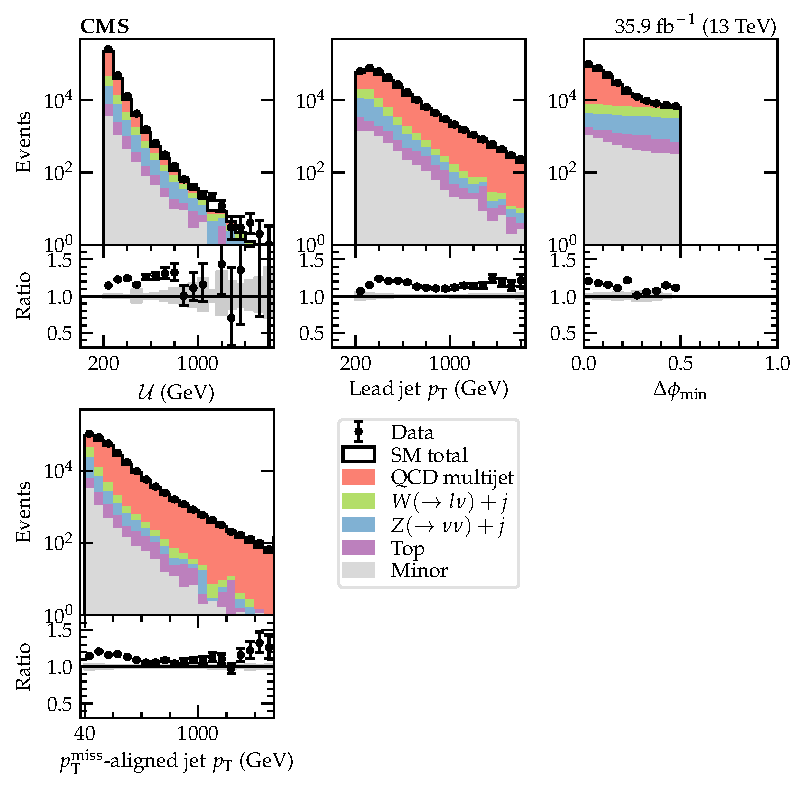
\includegraphics{chapters/042_backgrounds/images/monojetqcd_dists.pdf}
    \caption[QCD-enriched sideband kinematics.]{
        Kinematic distributions within the QCD-enriched sideband. The ratio is taken with respect to the SM total and includes the statistical uncertainty associated with the limited sample size.
    }
    \label{fig:monojetqcd-nearest-jet-pt}
\end{figure}
%
The sideband region predominantly consists of the QCD multijet process ($75.2\%$) with contamination from \IWlvj ($10.9\%$) and the signal \IZvvj ($9.5\%$), followed by a small contribution from $t$-quark and minor background processes ($4.3\%$).

A disagreement of $10$--$20\%$ between data and MC is not covered by scaling the \IWlvj process up by the $10\%$ determined from Sec.~\ref{sec:wjets-prediction}. Instead, this is attributed to mismodelling of the QCD multijet process. This disagreement is parameterised by a linear fit to the \pt distribution of the \ptmiss-aligned jet, extrapolated to the \metplusjets region at {$0$--$\SI{40}{GeV}$}, within each \recoil bin. A 2-dimensional fit is performed with the likelihood formalism (App.~\ref{app:likelihood}). The final six \recoil bins are combined to avoid categories of low statistical power. The linear fit is performed across 10 \ptmiss-aligned jet \pt bins from {$40$--$\SI{1040}{GeV}$}. The \IWj prediction is performed by the transfer factor method, discussed in Sec.~\ref{sec:wjets-prediction}, inclusive in the \ptmiss-aligned jet \pt.  Furthermore, the \IZvvj signal contamination within this region is allowed to vary to determine the correlation between the data-driven QCD multijet estimate and the \IZvvj signal. The postfit distribuition is shown in Fig.~\ref{fig:qcd_postfit}.
%
\begin{figure}
    \centering
    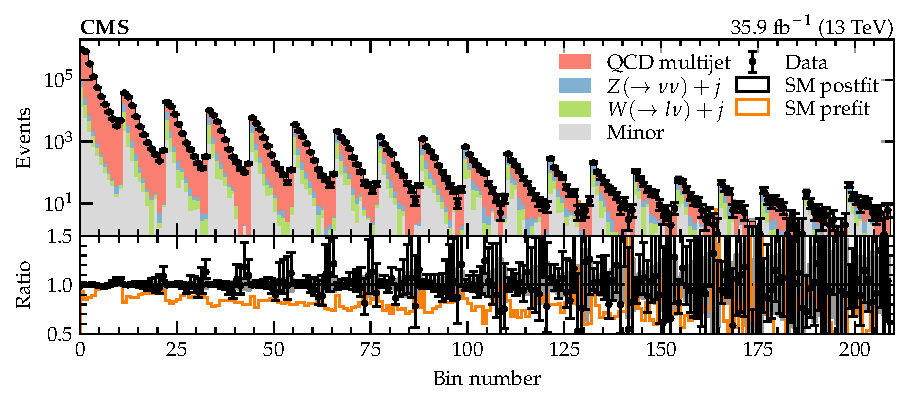
\includegraphics{chapters/042_backgrounds/images/qcd_postfit.pdf}
    \caption[QCD multijet estimation within the enriched sideband]{
        Postfit results of a fit to data in the QCD multijet enriched sideband allowing the normalisation on the \IZvvj and \IWlvj processes to vary and a linear shape variation on the QCD multijet process. The 2-dimensional binning is unfolded into 1-dimension labelled by the bin number, with $0$--$9$ corresponding to the \ptmiss-aligned distribution of the first \recoil bin, $10$--$19$ to the second \recoil bin, and so on for 19 \recoil bins in total. The ratio is taken with respect to the SM postfit result.
    }
    \label{fig:qcd_postfit}
\end{figure}
%
The parameterisation model introduced in the fit significantly improves the agreement between data and the prediction, with the extrapolation to the \metplusjets region shown in Fig.~\ref{fig:qcd_estimation}.
%
\begin{figure}
    \centering
    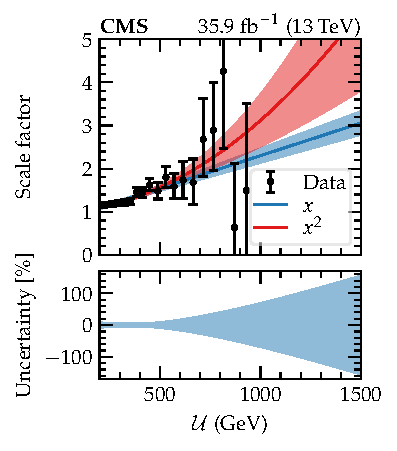
\includegraphics{chapters/042_backgrounds/images/qcd_estimation.pdf}
    \caption[QCD multijet scaling factor for the signal region.]{
        The QCD multijet scaling factor determined from a linear extrapolation from the QCD multijet enriched sideband to the \metplusjets region. The data points include the statistical and systematic uncertainties determined from the fit. Additional linear ($x$) and quadratic ($x^2$) fits are performed with the maximum difference taken as an uncertainty band, shown in the lower panel.
    }
    \label{fig:qcd_estimation}
\end{figure}
%
To a first order approximation, within uncertainties, the scale factors follow a linear trend with the \recoil. Therefore, a linear fit determines the scaling factor to the higher \recoil bins, with higher order effects determined from a quadratic fit taken as an uncertainty on the scale factors, ranging from a $5$--$100\%$ uncertainty on the correction. These corrections are applied as scaling parameters to the QCD multijet process within the \metplusjets region, with the uncertainty as alternative templates, decorrelated across the \recoil bins to allow the shape of the QCD multijet prediction to vary, as well as the normalisation. Furthermore, the predictions are found to have a $20\%$ anti-correlation with the \IZvvj normalisation, and hence this correlation is included within the final fit.


\section{\Pgstar contribution}

To determine the contributions to the \IDYll process from \IZll and \Igstarll, the processes are generated at NLO accuracy through the matrix element and parton shower, without the detector simulation to avoid the expensive computation. Regardless, the sample size of the generated \IZll and \Igstarll processes are limited and the statistical uncertainty, along with QCD scale and PDF variations, are propagated through the ratio of cross sections of both processes to the \IDYll interaction. The generated processes do not include any of the corrections discussed in Chap.~\ref{chap:simulation-corrections}, including the higher-order QCD and EW corrections since these will mostly cancel in the ratio of cross sections, with the small remainder estimated by the uncertainties. To avoid inconsistencies between various event generators, the 3 processes are generated by \MADGRAPH. The invariant mass distribution of the generator-level dilepton is shown in Fig.~\ref{fig:gstar_invmass}.
%
\begin{figure}
    \centering
    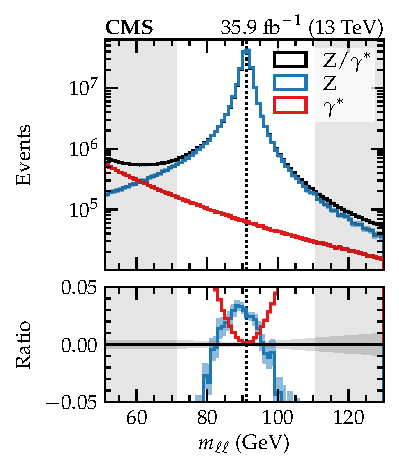
\includegraphics{chapters/042_backgrounds/images/gstar_invmass.pdf}
    \caption[Invariant mass distributions of the \IDYll, \IZll and \Igstarll processes.]{
        Invariant mass distributions of the generated dilepton from the \IDYll, \IZll and \Igstarll processes. The lower panel shows the ratio with respect to the \IDYll process, with the \IZll ratio subtracted by one to place it on the same scale as the \Igstar ratio. The uncertainty bands represent the statistical uncertainty of the MC samples. The region of interest, ${71<m_{\ell\ell}<\SI{111}{GeV}}$, is bounded by the grey regions.
    }
    \label{fig:gstar_invmass}
\end{figure}
%
The inclusive ratio of cross sections, with respect to the \IDYll process, within the fiducial region ${71<m_{\ell\ell}<\SI{111}{GeV}}$, defined by the analysis selection is used to determine the contributions from \Igstarll and the interference with the \IZll process. The \Igstarll component is treated as a background while the interference is treated as the \IZll signal scaled by the square-root of any signal strength modifiers, to account for the \IZll amplitude appearing in the interference cross section term. Therefore, within the likelihood to extract the \PZ invisible width, the contribution from the \IDYll process in the \diellplusjets region is
%
\begin{equation}
    \left(k_{\PZ}r_{\PZ} + (1 - k_{\PZ} - k_{\Pgstar})\sqrt{r_{\PZ}} + k_{\Pgstar}\right)s_{\IDYll}^{\diellplusjets}\ ,
\end{equation}
%
where $r_\PZ$ is the unconstrained parameter scaling the \IZll process, $k_{\PZ}$ is the constrained parameter measured from the ratio of \IZll to \IDYll cross sections, and $k_{\Pgstar}$ is similarly defined as the ratio of \Igstarll to \IDYll. An uncertainty associated with the extrapolation from the generator-level selection to the analysis region is performed by reweighting the distribution of partons initiating the interaction to the final analysis region. This captures effects caused by the analysis selection such as the lepton $\eta$ restriction and the high \recoil requirements. The values are determined after the reweighting procedure and the difference between the nominal result and the reweighted result is taken as a systematic uncertainty. The measured values are summarised in Tab.~\ref{tab:gstar-corrections}.

\begin{table}[htb]
    \centering
    \begin{tabular}{lll}
        \hline%\hline
        & $k_\PZ$ & $k_\Pgstar$ \\
        \hline
        Parameter value &  $1.0165$ & $0.0150$ \\
        MC Statistical uncertainty [\%] & $\pm 0.1$ & $\pm 0.1$ \\
        PDF uncertainty [\%] & $\pm 2.3$ & $\pm 2.4$ \\
        $\mu_F$ and $\mu_R$ uncertainty [\%] & - & - \\
        Reweighting uncertainty [\%] & $\pm 1.4$ & $\pm 13.5$ \\
        \hline%\hline
    \end{tabular}
    \caption[Contributions to the \IDYll from the \IZll and \Igstarll processes.]{
        The measured values for the $k_\PZ$ and $k_\Pgstar$ parameters with their associated systematic uncertainties. The factorisation and renormalisation scales have a negligible impact on these parameters.
    }
    \label{tab:gstar-corrections}
\end{table}


\section{Remaining backgrounds}

The remaining backgrounds in the \metplusjets and \diellplusjets regions are estimated directly from MC with all corresponding sources of systematic uncertainties included in the final fit to extract the \PZ invisible width.


\section{Summary}

The \IZvvj signal collected in the \metplusjets region is largely contaminated by the \IWlvj processes. This process is estimated through a data-driven prediction from the \ellplusjets control regions through the transfer factor approach. The consistency of the normalisation and shape of the \recoil distribution in the \muplusjets, \eleplusjets and \tauplusjets regions; as well as between the \mupplusjets and \munplusjets; is used to test the extrapolation from the control regions to the \metplusjets region performed in the transfer factor approach. The validation test results show a consistent set of control regions.

Although the QCD multijet process is a minor background within the \metplusjets region, the large cross section and difficulty in modelling the process has led to a data-driven estimate of this background. A MC-to-data correction is extrapolated from the QCD multijet sidebands through a linear fit to the \ptmiss-aligned jet \pt distributions. A further linear parameterisation determines the correction factor across the \recoil distribution, with an alternative quadratic fit to incorporate higher order effects along the \recoil distribution through a systematic uncertainty.

To determine the \PZ invisible width, the rate of the \IZll process is required. However, the \diellplusjets consists of the inseparable processes: \IZll, \Igstarll and their interference. Instead, these are estimated through a generator-level study where the \PZ and \Pgstar contributions are successively suppressed. Systematic uncertainties in this estimation include the theoretical PDF and QCD scale uncertainties, as well as the difference with the estimation under a reweighting of the partons initiating the interaction to the analysis reconstructed-level regions.

The estimation of these processes are used within the final fit to extract the rate of \IZvvj and \IZllj events to determine the \PZ invisible width.
